\chapter{神经网络与深度学习}

\section{数学基础与基本理解}
\subsection{深度与广度}
最基本的神经网络本质上就是一层套一层的连续变换

\begin{empheq}{align*}
\bm{y}&=\bm{f}_1(\bm{f}_2(\bm{f}_3\cdots(\bx)))\\
\bm{f}_i(\bx)&=\bm{\sigma}_i(W_i\bx+\mathbf{b}_i)
\end{empheq}

$\bm{\sigma}_i$就是激活函数,如果不加,那就是矩阵连乘.由于求导的链式法则,当导数小于1的时候,乘起来很快就变成0了,这是梯度消失;如果导数绝对值大于1,乘起来又可能变得很大,这是梯度爆炸.

激活函数一定要是非线性的,否则连续线性变换最终还是线性的.一般使用的激活函数是ReLU,它在大于0时是线性的,小于0时也是线性的.假如网络规模较小,比如就是传统的几层网络.那么当初始化后,假如恰好每一层的输出都大于0,那么就是线性的,此时梯度下降可能失效,导致最后训练出一个线性函数.此时必须引入更多的非线性.另一方面,只使用少数层可能使得所有输出大于0,但是假如提高深度,也可以增加非线性.

实际测试中发现,一个$1\rightarrow 5\rightarrow 10\rightarrow 1$的网络,如果全用ReLU激活函数,很容易习得一个线性函数,假如把其中一层改成ELU,那么就可以习得非线性.假如提高深度,中间中4层,那么也很容易习得非线性.这可能是说深度比广度更加重要一些.也说明网络效果与激活函数与初始化方式有关.


\paragraph*{为什么深度比广度更加重要}基本原因是用简单的事物来构造复杂的事物,一定要经过多次连续变换才行,即层次性.日常编程也是如此,需要对数据复合很多次才能得到目标结果.

从连续性的角度来理解,简单的事物,经过小的变换,是连续的,得到的新东西相比以前相差还不十分多,所以要经过很多变换才能得到目标.

在数学上,衡量一个函数的复杂性:极值的数量、不连续点的数量等等.

神经网络就是用简单的函数来逼近复杂的函数:加法、乘法、基本函数.


\paragraph*{连续变换} 从信息论的角度讲,做变换就可能造成信息损失,所以整个网络的表达能力取决于中间层的最小宽度和深度.

为什么残差网络有用,连续变换过程中丢失了信息,现在把原来的信息再传一遍,起到了一个增强的作用.

从表示论的角度中,中间层就是用一种新形式来表达原来的输入.这就与所谓的流形学习有关——现实中的高维数据通常可以用更小的维度来表达.

非光滑函数经过变换,通常还是非光滑的,这启示我们如果想逼近光滑函数,应该用光滑激活函数如$\tanh x$.如果想逼近非光滑的函数,如分类问题,应该用非光滑激活函数如$\ReLU,\HardTanh$.

连续线性变换,还是线性变换,包括卷积在内都属于线性变换.

\subsection{理解非线性}
非线性有不同的类型,比如对于CV来说,非线性可能是指Piecewise的非线性,就是分为很多段,但在局部仍然是接近线性的.在这种情形下,用ReLU就非常合适,因为它本身就适合描述if else判断.

有的非线性是指在整个区间上光滑,但是不同局部的增长速度不同.增长速度大致可以分为多项式或者指数级.可以设想,对于指数增长,用ReLU可能就不合适,因为复合线性乘法,本质上是多项式增长的,没法实现指数增长.

在这样的理念引导之下,我们可以设想,假如拟合超过多项式增长的函数,就引入一层指数函数.

非线性中尤其强调离散,注意离散是非线性,常用的Bool逻辑就属于离散函数.

\subsection{用神经网络表达各种函数}
\subsubsection{$\max$}
二维时:
$$\max (x,y)=\ReLU (x-y)+y$$

$n$维时,有几种思路.比如第一种:每次比较两个,选最大的,进行$n-1$次比较选出最大值,这样构造出来有$n-1$层.或者构造一棵树,一次比较$n/2$对,需要$n/2$层.

\subsubsection{两段直线}
\[
f(x)=\begin{cases}
	\frac{1}{3}x&,\ \text{if} x<=0 \\
	x&,\ \text{otherwise}
\end{cases}
\]

原点左边斜率为$\frac{1}{3}$,右边为$1$.这可以用$\ReLU$与$\sign$合成:
\begin{empheq}{align*}
f(x)&=\frac{1}{3}x+\frac{2}{3}\ReLU x\\
&=-\frac{1}{3}\sign (x) x+\frac{4}{3}\ReLU x
\end{empheq}


\subsection{作为核方法的深度学习}
有文章指出:使用梯度下降法学习的模型本质上近似于核方法\ref{deep_learning_as_ker}。所谓核方法就是简单地记忆数据,然后在遇到新样本时,通过查询、整合相似的记忆来输出结果。

本文中认为核心方法形如:
$$y=g\sbra{\sum_i a_i K(x,x_i)+b}$$
$g$为非线性函数,$a_i$为参数,在监督学习中通常就是$y_i$。$x_i$为已有样本,所以这是在说$x$的结果是其它样本的结果按相似度进行组合。

文章中提出了两种核
\begin{empheq}{align*}
K_{f,v}^g(x,x')&=\nabla_wf_w(x)\cdot \nabla_wf_w(x') \mtag{Tangent Kernel}\\
K_{f,c}^p(x,x')&=\int_{c(t)}K_{f,w}^g(x,x')\dif t \mtag{Path Kernel}
\end{empheq}


但文章也指出,一个SVM相当于单层的神经网络。而深度学习模型并不能简单地化简为核方法,因为它相比浅层网络可以表示指数级的复杂度,只是使用梯度下降法学习的模型相当于核方法。

\subsection{完备基函数组与参数效率、表达能力}\label{neural-network-basis-function}
神经网络是在用一些基本的Building block搭建整体,那么所选择的building block必定要具有某种“完备性”,才能具有足够的表达能力。一个简单的例子是用全连接层是很难表达$y=x_1x_2$的,全连接层的基本模型是
$$y=A_3\sigma(A_2\sigma(A_1\bx+\bm{b}_1)+\bm{b}_2)+\bm{b}_3$$
如果抛开激活函数不看,那么输出就是线性组合,并不存在输入之间的边乘项,猜想是不能准确地表达$x_1x_2$。

以下说明完全基函数组,首先是二元运算:
\begin{description}
\item[矩阵乘法] 内积$\cdot$也属于矩阵乘法。
\item[加法+]
\item[element-wise乘法$\otimes$]
\item[拼接Concatenate$\|$]
\end{description}
再配上激活函数或者一些一元运算:
\begin{description}
\item[$\min,\max$] $\ReLU$激活函数可以表达这两种。
\item[$\exp$]
\item[$\text{pow}$] 乘方。
\item[复制] 复制这个操作一般是隐含的,比如在卷积网络中,输入一个图片,可以用多个Features卷积产生输出,其实就包含了复制操作。
\item[缩放] 标量乘法。softmax可以由$\exp$与缩放复合而成。
\end{description}

二元运算虽然比较少,但是分左和右。神经网络的信息分参数与输入,那么每种运算至少有$(2+1)\times(2+1)=9$种可能,一下就非常多了。2和1是指参数与输入,1是指混合,不过只有参数与参数运算,意义不大,去掉这一种,至少也有8种。同时参数与输入还有顺序关系,比如残差层使用了之前的输出,可能的情况会更多。

观察大多数神经网络,都使用了以上结构,Transformer可能是最复杂的,基本把以上都包含了。

\subsection{拟合指数增长函数}
拟合指数增长函数并不是一件容易的事。首先一般的线性模型、多项式模型都无法做到,无论使用何种分布假设、使用马尔科夫链。神经网络中假如使用$\ReLU$激活函数,那么本质上是局部线性的,也不可能准确拟合指数增长函数。

有几种思路,要么改进模型,增加相应的基函数组,要么对数据进行变换,使之线性化。比如对数据取$\ln$变换。变换的思路可以应用于神经网络中,比如中间某一层,首先取$\ln(\ReLU(x)+1),\ln(\text{sigmoid}(x))$,经过线性组合后,再取$\exp$,如果直接使用$\exp$可能出现溢出。

金融领域中,有些股票的价格就是呈现指数增长状态的。

对于分类模型而言,随着深度的增加,树的分支也是呈现指数增长的,这种指数增长不能通过取对数来处理。使用传统的神经网络模型显然无法准确地处理,这也是研究双曲神经网络的一个重要原因,它适用于描述指数增长。

\subsection{初始化}
\subsubsection{Kamming}
\begin{equation}
W=U/\sqrt{out/2}
\end{equation}
以上中$out$表示输出的大小。
\section{各种神经网络层}
\subsection{Convolution}
Convolution就是局部元素的线性组合,相当于把全连接层拆分.假如对一个序列自身进行Convolution,就是自回归,两个序列进行Convolution,就是线性回归.以下说明一些基本概念.

\paragraph*{channel}Chanel本来是图像中的概念,比如一般的彩色图片有三个Channel,每个Channel是一个矩阵.对于1D的情形,输入向量$n\times1$,可以视为1个Channel.

\paragraph*{padding}在1D的情形,假如序列长度为$n$,取长为$k$的核,那么输出为$n-k+1$,长度缩短了,需要在输入的两边补充0元素来使输出进行扩张.

\paragraph*{stride}每次核移动多少距离,一般是取1.移动的距离越短,则输出越少.

\paragraph*{dialation}间距.一般是取连续的元素与核进行合成,现在用不连续的元素来合成,就是dialation.

\paragraph*{group}默认是1,要求in\_channels和out\_channels是它的倍数.核的数量=in\_channels/groups*out\_channels.见下图.使用分组可以直到截断关联的作用.取分组为1的时候,输出的每个Channel是由所有输入的channel复合而成.如果取分组为in\_channel,那么就叫depth-wise convolution,每个in\_channel展开成多个out\_channel.

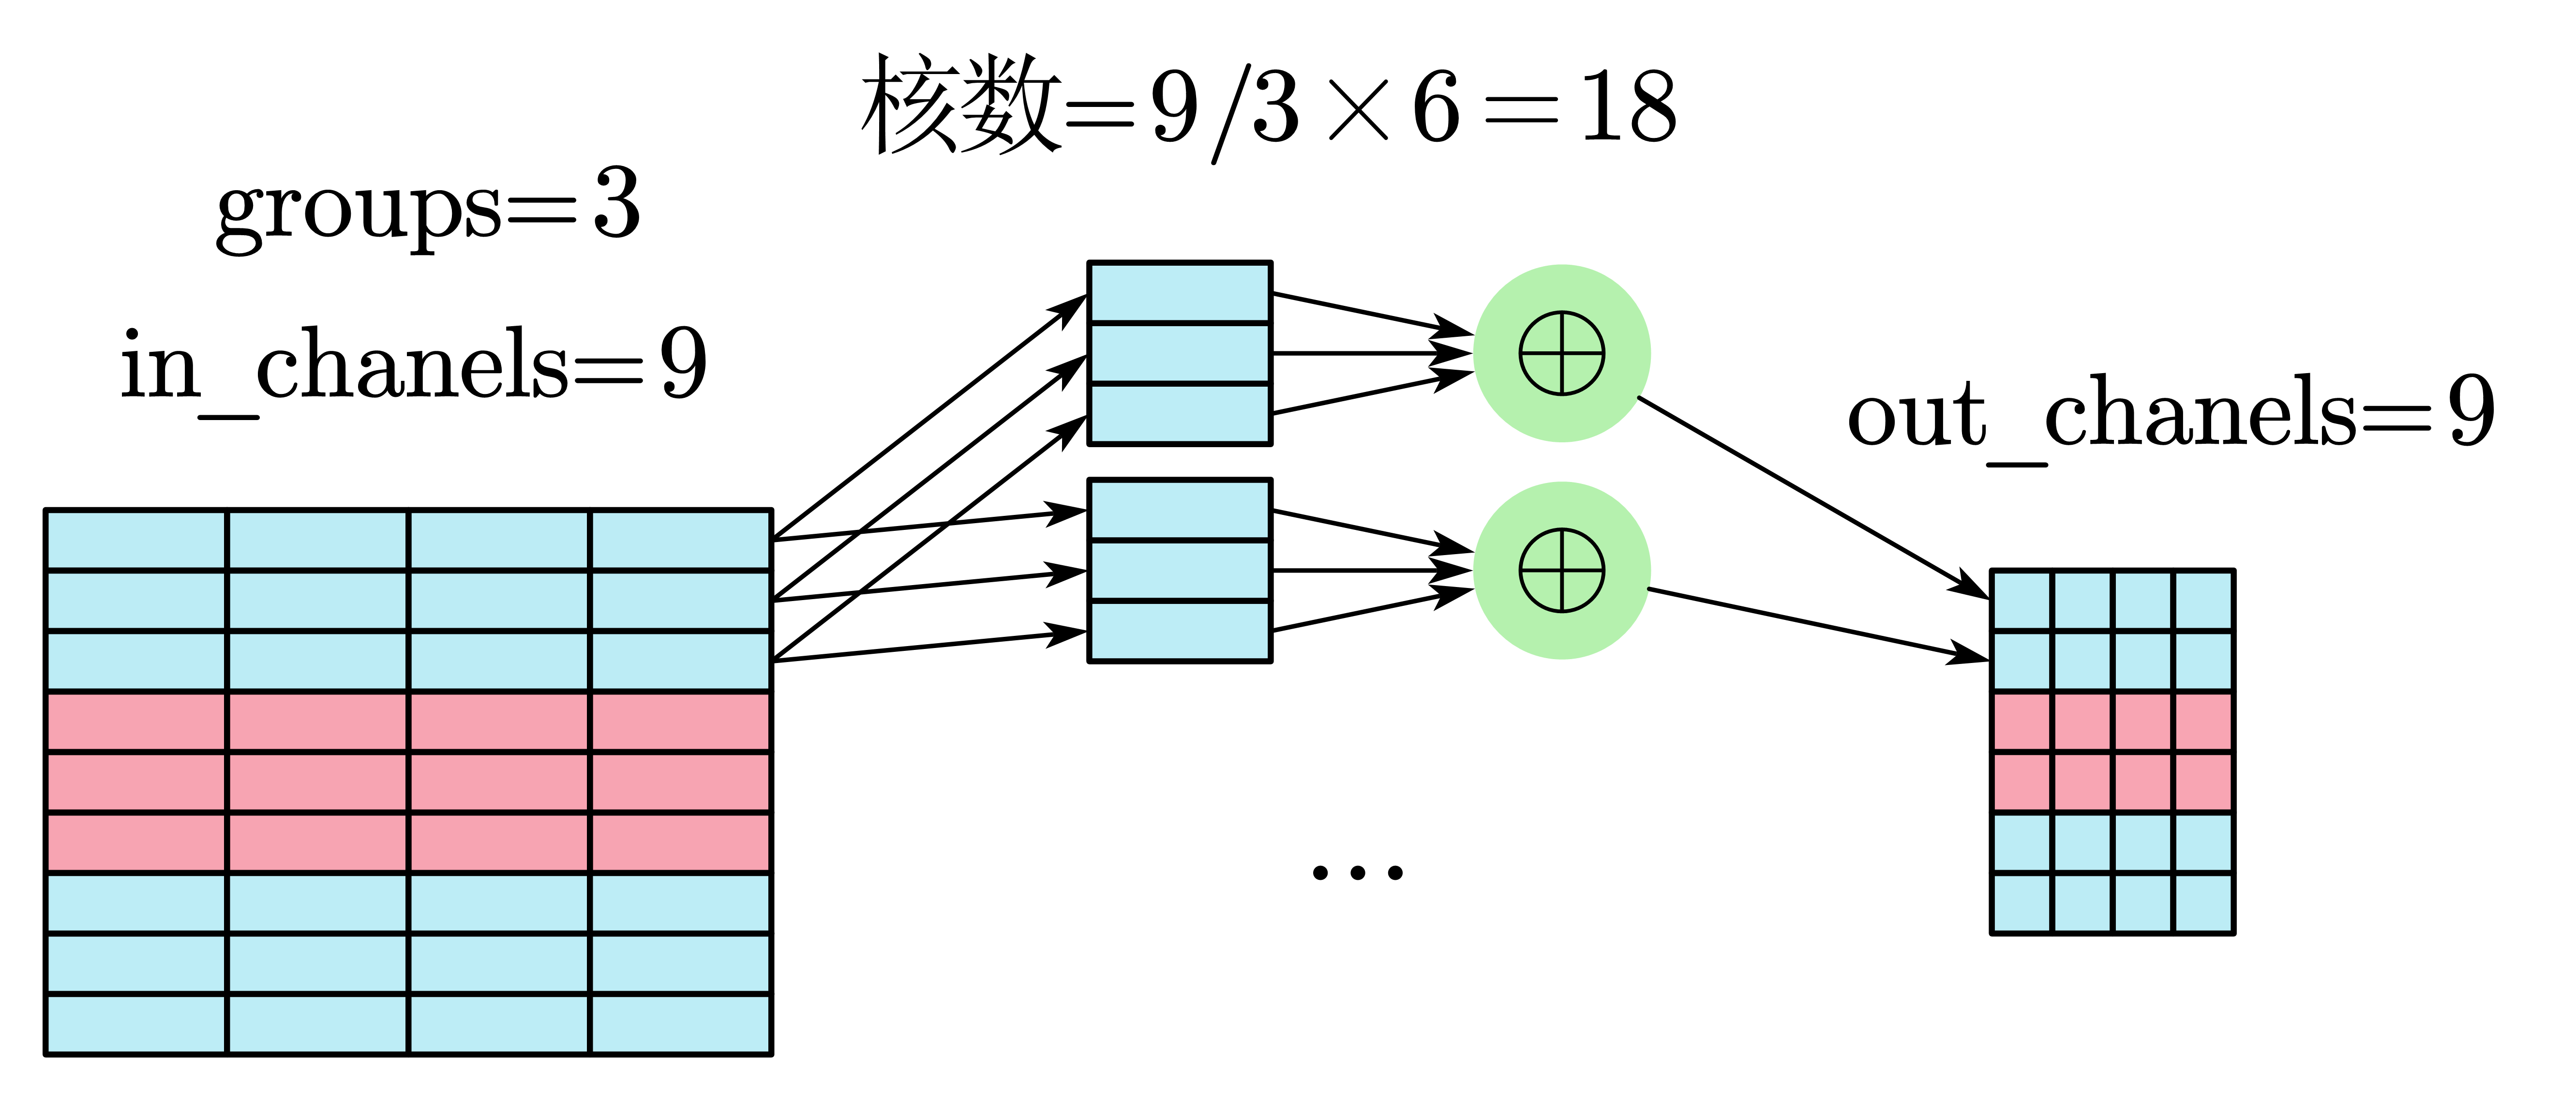
\includegraphics[width=\textwidth]{figure/Convolution-Groups.png}

注意图中,左边每次滑动移动距离为窗长,实践中一般是移动1.显然,Convolution捕捉的是局部相关性,因为它把相邻近的元素进行组合.

\subsection{LSTM层}
\subsubsection{数学表达式}

\begin{empheq}[left=\empheqlbrace]{align*}
\widetilde{\bm{c}}_t&=\tanh (W_c\bx_t+U_c\bm{h}_{t-1}+\bm{b}_c)\\
\bm{i}_t&=\sigma(W_i\bx_i+U_i\bm{h}_{t-1}+\bm{b}_i)\\
\bm{f}_t&=\sigma(W_f\bx_t+U_f\bm{h}_{t-1}+\bm{b}_f)\\
\bm{o}_t&=\sigma(W_o\bx_t+U_o\bm{h}_{t-1}+\bm{b}_o)\\
\bm{c}_t&=\bm{f}_t\odot\bm{c}_{t-1}+\bm{i}_t\odot\widetilde{\bm{c}}_t\\
\bm{h}_t&=\bm{o}_t\odot\tanh(\bm{c}_t)
\end{empheq}

\subsubsection{示意图}
一个LSTM Cell的结构如下图所示,图中的$N$表示输入(Batch Size为1,为向量,对应于Features或者Channel个数)的长度,$M$是Hidden size。

\begin{center}
\includegraphics[width=12cm]{figure/LSTM Cell.png}
\end{center}

可以从图中看出,参数的个数是$\underbrace{(M+N)\times N \times 4}_{\text{四个门的矩阵乘法}}+\underbrace{(M+N)\times 4}_{\text{四个门的偏移}}$。

一个LSTM层由多个LSTM Cell堆叠起来。整个层的输入通常是$(N,L,C)$,每次取1列送往网络进行计算,则每次的输入是$(N,C)$,最终的输出是$(N,C_H)$。如下图所示:

\begin{center}
	
\includegraphics[width=12cm]{figure/LSTM Sample.png}
\end{center}

\subsection{GRU层}
\subsubsection{数学表达式}
\begin{empheq}[left=\empheqlbrace]{align*}
\bm{h}_t&=\bm{z}_t\odot\bm{h}_{t-1}+(1-z_t)\odot \widetilde{\bm{h}}_t\\
\bm{z}_t&=\sigma(W_z\bx_t+U_z\bm{h}_{t-1}+\bm{b}_z)\\
\widetilde{\bm{h}}_t&=\tanh (W_h\bx_t+U_h(\bm{r}_t\odot\bm{h}_{t-1})+\bm{b}_h)\\
\bm{r}_t&=\sigma(W_r\bx_t+U_r\bm{h}_{t-1}+\bm{b}_r)
\end{empheq}
\subsubsection{示意图}

\begin{center}
\includegraphics[width=12cm]{figure/GRU cell.png}
\end{center}

\subsection{Residual层}
\subsubsection{数学表达式}
\begin{empheq}{align*}
\by&=\mathcal{F}(\bx)+\bx
\end{empheq}

\subsubsection{示意图}
\begin{center}
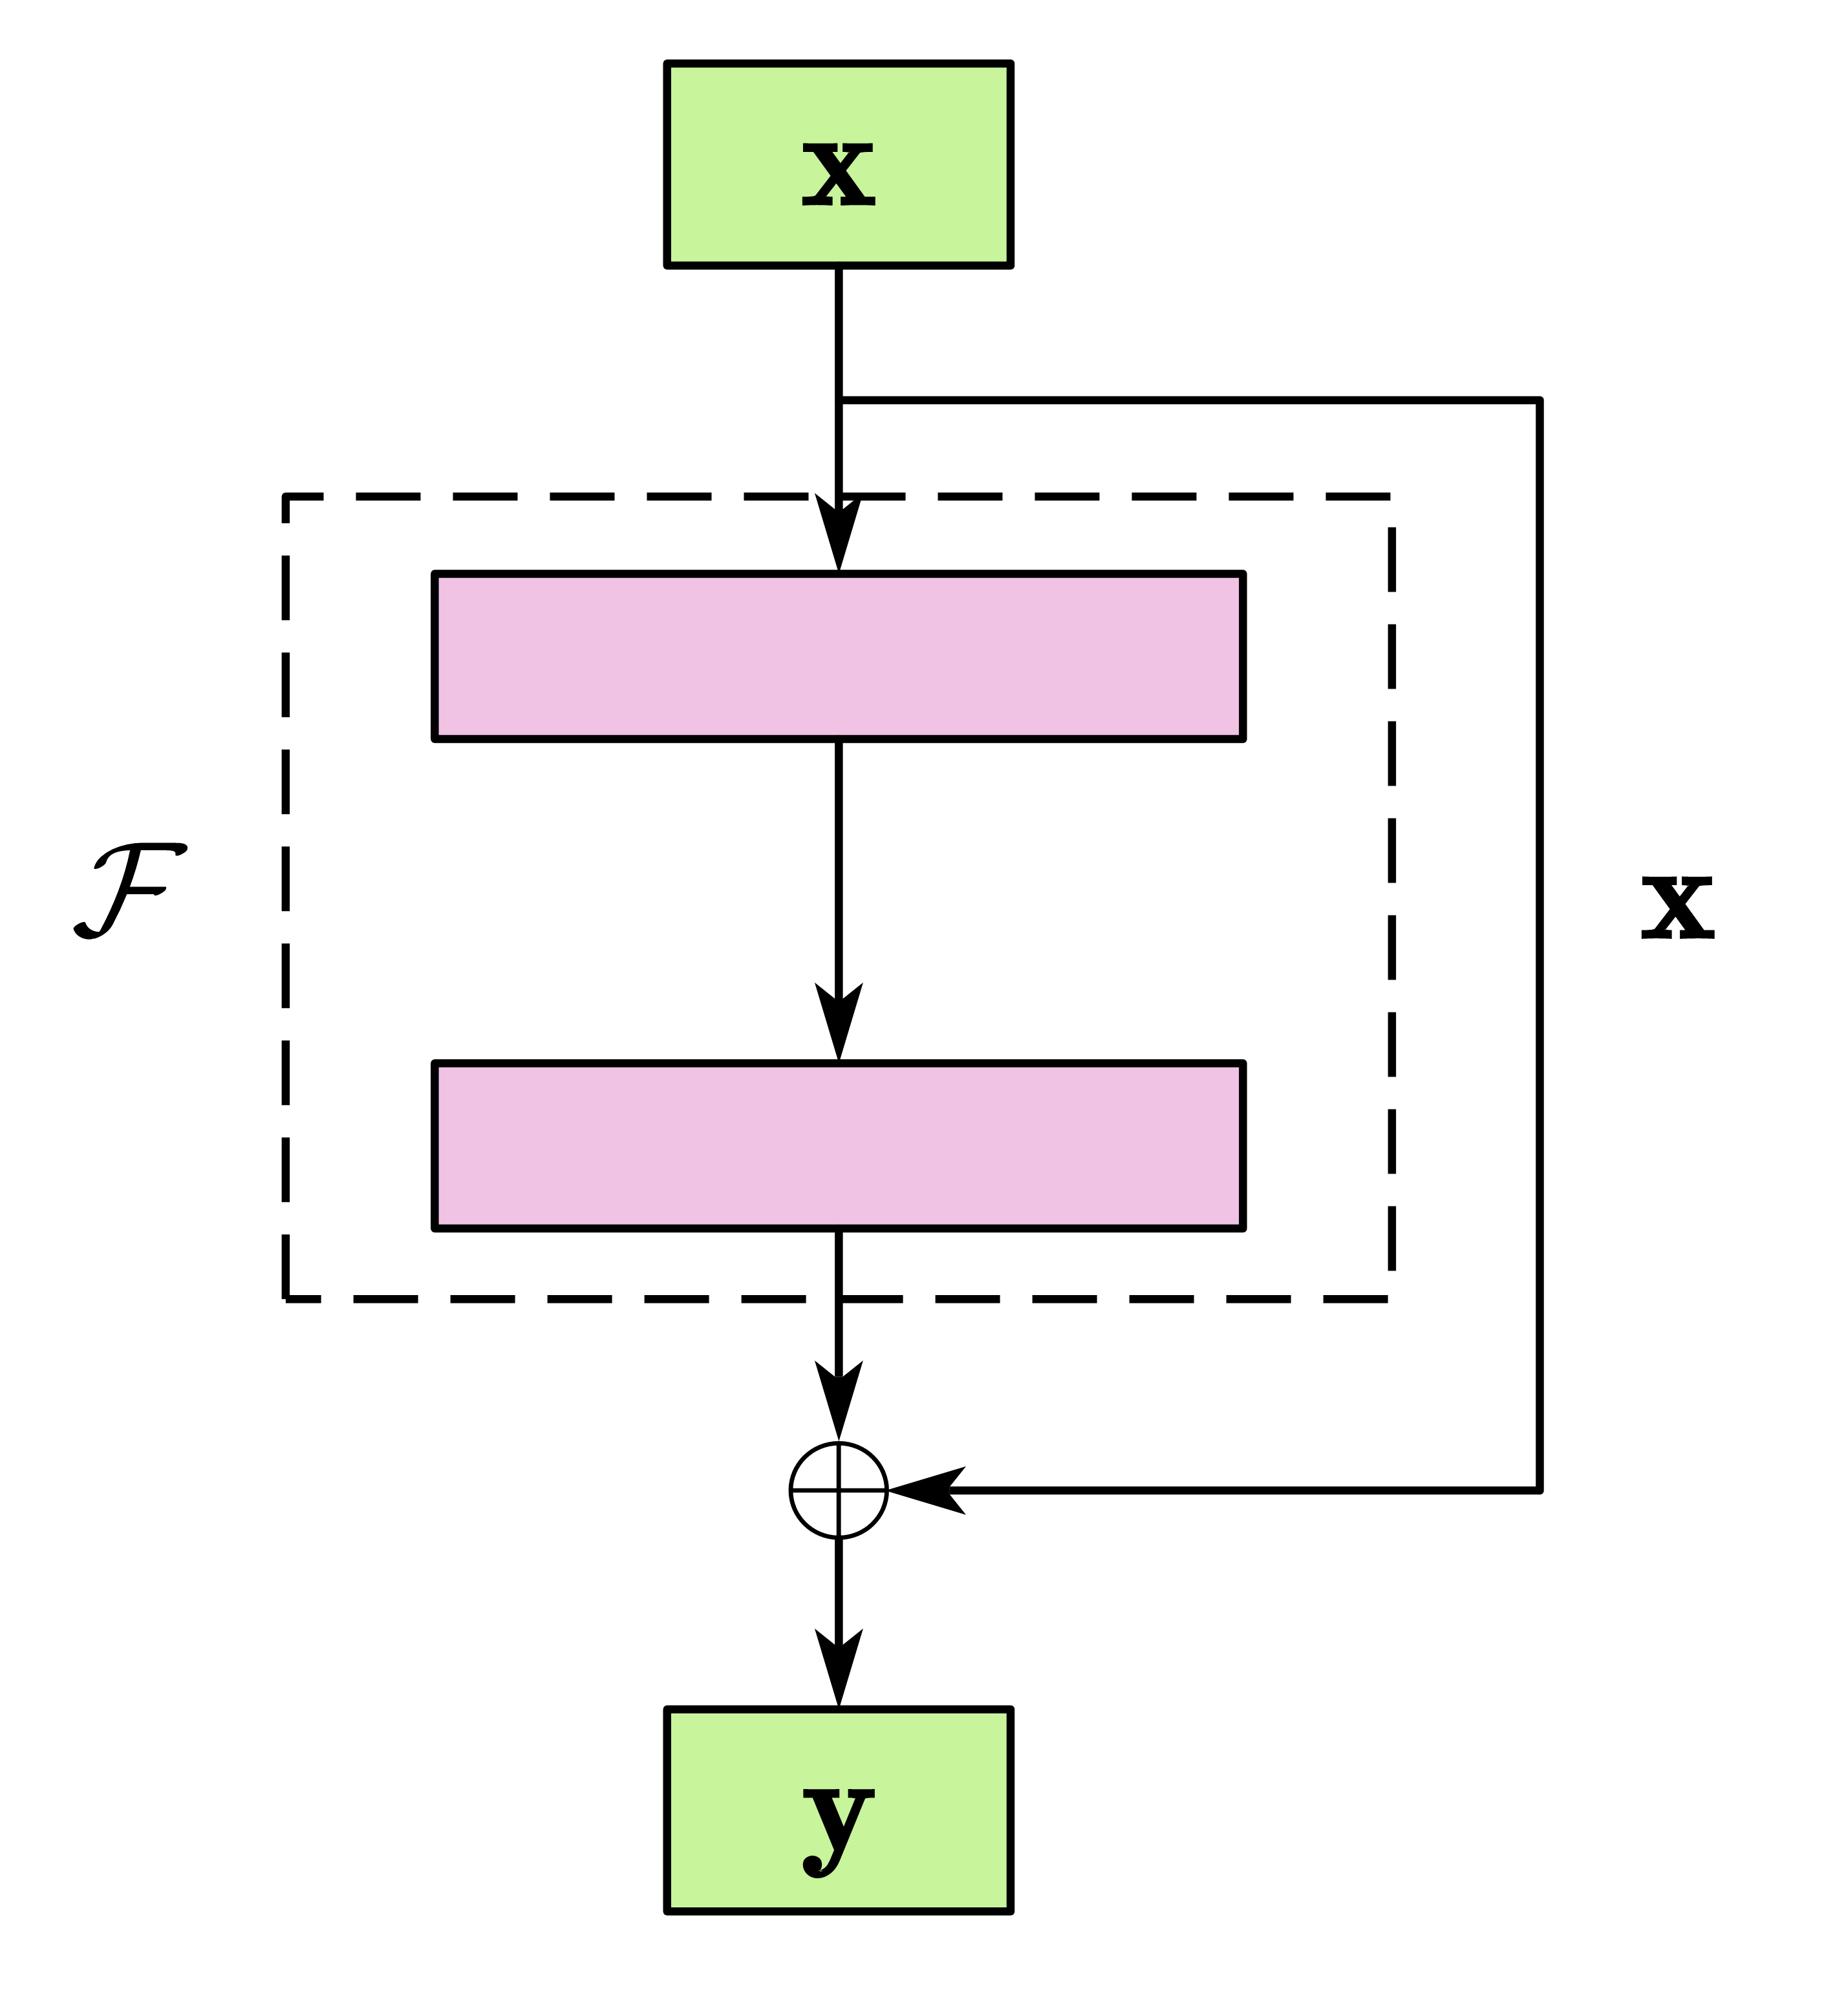
\includegraphics[width=6cm]{figure/Residual-block.png}
\end{center}

从图中可以看出,所谓残差是指
$$\mathcal{F}(\bx)=\by-\bx$$

此外,直接将输出传送到输出,也叫identity map by shortcuts,所谓identity就是指$\bx$.

\section{各种损失函数}


\section{各种激活函数}
注意$\sign$也可以用作激活函数.
\subsection{ReLU族}
特征是在输入小于0时输出接近0,而大于0时保持。

\subsubsection{ReLU}
函数形式:
\[
ReLU(x)=\begin{cases}
	0&,\ \text{if} x<=0 \\
	x&,\ \text{otherwise}
\end{cases}
\]

同时$\ReLU$也可以用$\sign$表达:
$$\ReLU(x)=\frac{1}{2}(\sign(x)+1)*x$$

\pgfplotsset{
	myplot/.style={
		width=8cm, height=4cm,
		xlabel=$x$, ylabel=$ReLU(x)$,
		samples=50,
		xlabel style={at={(1,0)}, anchor=west},
		ylabel style={rotate=-90, at={(0,1)}, anchor=south west},
		legend style={draw=none, fill=none},
		xmin=-3, xmax=3
	}
}
\begin{center}
	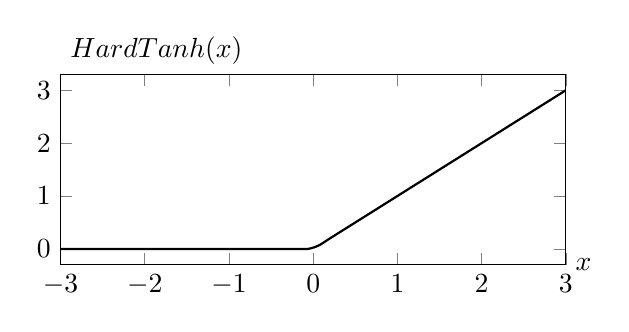
\begin{tikzpicture}[>=stealth,
		every node/.style={rounded corners},
		declare function={
			ReLU(\x)=((\x>0)*\x);
		}]
		
		\begin{axis}[myplot]
			\addplot[smooth, thick, domain=-3:3] {ReLU(x)};
		\end{axis}
	\end{tikzpicture}
\end{center}
\subsubsection{LeakyReLU}
ReLU加强版,负数不归0,而是用一条小斜率的直接取代.
\[
LeakyReLU(x)=\begin{cases}
	slope\times x&,\ \text{if} x<=0 \\
	x&,\ \text{otherwise}
\end{cases}
\]

$slope$在Pytorch中默认为0.01.
\subsubsection{PReLU}
LeakyReLU加强版,允许对输入为负数时的斜率进行学习:
\[
PReLU(x)=\begin{cases}
	ax&,\ \text{if} x<=0 \\
	x&,\ \text{otherwise}
\end{cases}
\]

$a$为一可学习的参数.按Pytorch官方的说法,使用这个激活函数时,不要用权重衰减.

\subsubsection{RReLU}
类似于PRELU,允许对输入为负数时的斜率进行学习:
\[
RReLU(x)=\begin{cases}
	ax&,\ \text{if} x<=0 \\
	x&,\ \text{otherwise}
\end{cases}
\]

$a$为随机采样的斜率.函数形式与RReLU完全一样。

\subsubsection{GeLU}

在Transformer中经常使用。

\[
\text{GeLU}(x)=x\Phi(x)
\]

\pgfplotsset{
	myplot/.style={
		width=8cm, height=4cm,
		xlabel=$x$, ylabel=$\text{GeLU}(x)$,
		samples=50,
		xlabel style={at={(1,0)}, anchor=west},
		ylabel style={rotate=-90, at={(0,1)}, anchor=south west},
		legend style={draw=none, fill=none},
		xmin=-3, xmax=3
	}
}
\begin{center}
	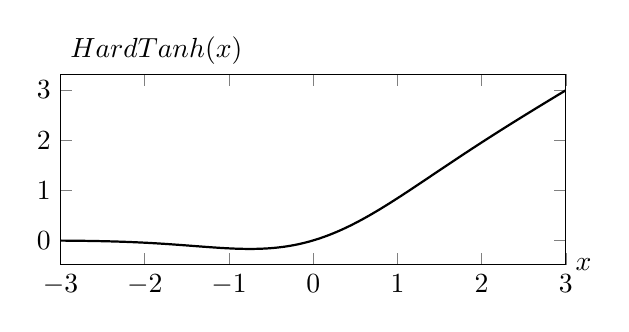
\begin{tikzpicture}[>=stealth,
		every node/.style={rounded corners},
		declare function={
			GeLU(\x)=x/(1 + exp(-0.07056*pow(\x,3) - 1.5976*\x));
		}]
		
		\begin{axis}[myplot]
			\addplot[smooth, thick, domain=-3:3] {GeLU(x)};
		\end{axis}
	\end{tikzpicture}
\end{center}

\subsection{tanh族}
特征是输出有界。

\subsubsection{tanh}
\pgfplotsset{
	myplot/.style={
		width=8cm, height=4cm,
		xlabel=$x$, ylabel=$tanh(x)$,
		samples=50,
		xlabel style={at={(1,0)}, anchor=west},
		ylabel style={rotate=-90, at={(0,1)}, anchor=south west},
		legend style={draw=none, fill=none},
		xmin=-3, xmax=3
	}
}
\begin{center}
	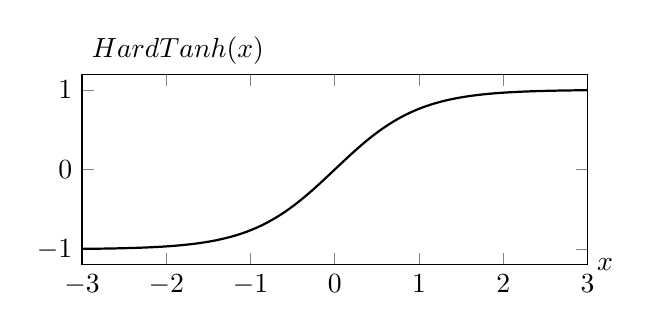
\begin{tikzpicture}[>=stealth,
		every node/.style={rounded corners},
		declare function={
			tanhf(\x)=tanh(x);
		}]
		
		\begin{axis}[myplot]
			\addplot[smooth, thick, domain=-3:3] {tanhf(x)};
		\end{axis}
	\end{tikzpicture}
\end{center}

\subsubsection{HardTanh}
函数形式:
\[
ReLU(x)=\begin{cases}
	-1&,\text{ if } x\leq-1 \\
	x&,\text{ if } -1\leq x\leq 1 \\
	1&,\text{otherwise}
\end{cases}
\]

\pgfplotsset{
	myplot/.style={
		width=8cm, height=4cm,
		xlabel=$x$, ylabel=$HardTanh(x)$,
		samples=50,
		xlabel style={at={(1,0)}, anchor=west},
		ylabel style={rotate=-90, at={(0,1)}, anchor=south west},
		legend style={draw=none, fill=none},
		xmin=-3, xmax=3
	}
}
\begin{center}
	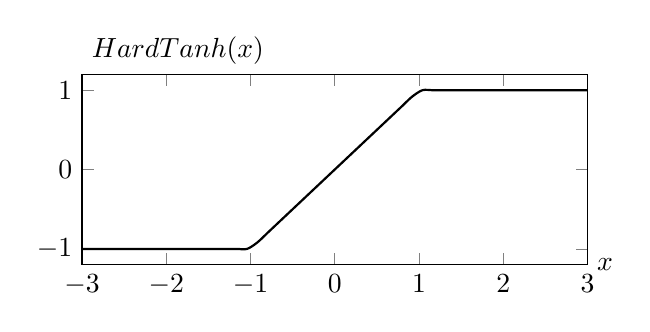
\begin{tikzpicture}[>=stealth,
		every node/.style={rounded corners},
		declare function={
			HardTanh(\x)=((\x>1)+(\x<-1)*(-1)+and(\x<1,\x>-1)*x);
		}]
		
		\begin{axis}[myplot]
			\addplot[smooth, thick, domain=-3:3] {HardTanh(x)};
		\end{axis}
	\end{tikzpicture}
\end{center}

\subsection{Huber族}
\subsubsection{Huber Loss}
$$L_\delta(x)=\begin{cases}
\frac{1}{2}x^2&\text{ if } |x|\leq \delta \\
\delta x-\fh\delta^2 & \text{ otherwise }
\end{cases}$$
可以自然地拓展到进行函数逼近:
$$L_\delta(y,f(x))=\begin{cases}
	\frac{1}{2}(y-f(x))^2&\text{ if } |y-f(x)|\leq \delta \\
	\delta|y-f(x)|-\fh\delta^2 & \text{ otherwise }
\end{cases}$$

在靠近0的小区域内,它是二次的,在外面,它是线性的。而且本函数是光滑的。

\subsection{归一化类}
\subsubsection{softmax类}
\paragraph*{原始softmax}可以用来限定和为1,且值为正数,因此用来表示概率。
$$\softmax(x_i)=\frac{\exp(x_i)}{\sum \exp(x_i)}$$

\paragraph*{log-softmax}
$$\text{log-softmax}(\bx)=\ln(\softmax(\bx))\approx \bx-\max(\bx),x_i\in(-\infty, 0]$$
$\sum \exp(x_i)$会被,较大的数所主导,所以$\ln\left(\sum x_i\right)\approx \max (\bx)$。
\paragraph*{其它变体}
\begin{enumerate}
	\item 限定和为1,且有正负:$$n\softmax(\bx)-\frac{n-1}{n},x_i\in\left(-\frac{n-1}{n},n-1+\inv{n}\right)$$可以用来表示可以做空的投资权重。另一种方式是直接用绝对值归一化:
$$\frac{\bx}{\sum |x_i|},x_i'\in[-1,1]$$
但这种表示方法是仅仅绝对值之和为1,和是不确定的,而且因为有除法,不容易训练。
\item 在上一种方法上进行扩展:
$$a\softmax(\bx)-\frac{a-1}{n}$$
值域为
$$	x_i\in\begin{cases}
\left(-\frac{a-1}{n},\frac{n-1}{n}a+\inv{n}\right),&\text{if } a>0\\
	\left(\frac{n-1}{n}a+\inv{n}, -\frac{a-1}{n}\right) &\text{if } a<0
\end{cases}$$
\begin{note}
	\begin{enumerate}
		\item 如果希望限定最大值,比如对于3个数,取
		$$a-1+\frac{1}{n}\leq 1\implies a\leq \frac{3}{2}$$
		假如令$a=\frac{3}{2}$,则$x_i'\geq -\inv{2n}$,非常接近0了,不算太理想。
		
		要使下界小于0,必然有$a\geq 1$,上界$\geq \inv{n}$。
		\item 区间的长度为$\lvert\frac{n+1}{n}a-1\rvert$。
		\item 如果希望区间对称,则$\frac{a-1}{n}=\frac{n-1}{n}a+\inv{n}$,此时$a=\frac{2}{2-n}<0\rightarrow 0,x_i'\in\left(-\inv{n-2},\inv{n-2}\right)$,对于3个数,取$a=-2$,则区间为$(-1,1)$,这比较理想。如果$n=10,a=-\inv{4},x_i'\in\left(-\inv{8}, \inv{8}\right)$,不太理想。这个变换界卡得太死了。
		\item 由于$\softmax$值域是大于0的,线性变换要使区间对称,必然需要左偏,则$a<0$。
	\end{enumerate}

\end{note}
\end{enumerate}
\subsubsection{有界投影法}
考虑这样一种操作,首先把输出变换成有界区间$[a,b]$,再投影到平面$\sum x_i=1$平面上,由于输入有界,则投影后也有界,而且这个界易于自己控制。这样得到的结果是:
\begin{equation}\label{constrained-projection-normalize}
x_i'=\frac{1-\sum x_i}{n}+x_i
\end{equation}
这个变换的矩阵表示为:
$$\bx'=\left(I-\inv{n}\bm{1}_{n\times n}\right)\bx+\inv{n}\bm{1}_{n\times 1}$$
这个矩阵是不可逆的。

注意到\ref{constrained-projection-normalize}是一个线性变换,它会把极点变换成极点,但$[-a,\bm{0}]$显然不是极点,所以不应该代入这个。应该取$[-b,\bm{a}]$和$[a,-\bm{b}]$,输出界为
$$\left[\inv{n}-\frac{-b+(n-1)a}{n}-b,\inv{n}-\frac{a-(n-1)b}{n}+a\right]$$
仍然不对称。而且注意到,上下界之和为$\frac{2}{n}$,因此必然不可能对称,不过在$n$比较大时,差别就很小了。

如果约束上界为$u$,为方便计算,取$a=b$,那么解得
$$a=b=\frac{nu-1}{2n-2}$$
在$u=1$时,$a=b=\inv{2}$,此与维度无关,下界为$\frac{2}{n}-1$。
\section{各种网络结构}
\subsection{GAN}
\subsubsection{原始GAN}
原始GAN模型\cite{goodfellow2014generative}由两个部分组成:生成器、判别器。前者的任务是从先验(通常取均匀分布或者高斯分布)中生成服从目标分布的数据,而判别器的任务是判断生成的数据是否符合目标分布。从结果上看,生成器起到了将先验分布变换为目标分布的作用。图示如下:

\begin{center}
	
\includegraphics[width=15cm]{GAN.png}
\end{center}

如图所示,模型更新过程分为两个步骤,首先更新判别器,使用的是梯度上升,极大化目标函数。理想情况下$D(x)\rightarrow 1,D(G(z))\rightarrow 0$。需要注意的是,判别器是一个二分类器,输入只有1个,判断这个样本是不是目标分布,并非输入为2个。


再更新生成器。更新生成器时,进行梯度下降使用的样本是新生成的样本,并非第一步里面生成的样本。

从更新过程中可以看出,判别器不是越强越好。假如判别器的能力是无限的,那么$D(G(z))=0$,第二步更新生成器的过程就没有用了。

实际来看,GAN是比较难训练的。推荐以下策略:
\begin{enumerate}
\item 学习率不能太低,大概可以设成1e-5这样。可以使用衰减策略。
\item 分类器的学习率可以设成比生成器学习率低,一般可以取后者的1/10。
\item 
\end{enumerate}

\subsubsection{应用GAN}
\paragraph*{时间序列预测}下图来自\cite{ZHANG2019400}。模型结构如图所示:
\begin{center}
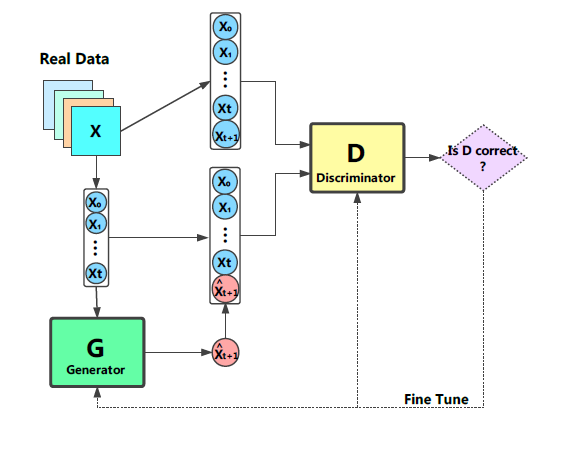
\includegraphics[width=10cm]{figure/gan-in-stock-pred.png}
\end{center}

核心在于生成器给出前向预测。

\subsection{Transformer}

\subsubsection{网络参数结构}
pytorch中,一个
\begin{verbatim}
	torch.nn.Transformer(d_model=10, nhead=5,dim_feedforward=200)
\end{verbatim}
的参数数量为59080。默认构造函数的参数是num\_encoder\_layers =num\_decoder\_layers=6。网络参数结构如下:
\begin{empheq}{align*}
\underbrace{\begin{bmatrix}
	300 & 30 & 100 & 10 \end{bmatrix}}_{\text{Multi-head Attention}}\underbrace{\begin{bmatrix} 2000 & 200 & 2000 & 10\end{bmatrix}}_{\text{FF}}\begin{bmatrix}
	10\times 4
\end{bmatrix}
\times 6 &=28140\\
\begin{bmatrix}
10
\end{bmatrix} &=5\\
\begin{bmatrix}
10&10 &	300 & 30 & 100 & 10 &300 & 30 & 100 & 10\end{bmatrix}
\underbrace{\begin{bmatrix} 2000 & 200 & 2000 & 10\end{bmatrix}}_{\text{FF}}
\begin{bmatrix}
10\times 4
\end{bmatrix}\times 6&=14850\\
\begin{bmatrix}
10\times 4
\end{bmatrix}&=15\\
&=28940
\end{empheq}

\subsubsection{示意图}
Transformer可以调用现成的库作为层调用,但其实内部比较复杂,更接近架构的概念,而非普通的层。表示为
$$(L_1,N,C)\times (L_2, N, C)\rightarrow (L_2, N, C)$$

此处引用一张广为流传的图:
\begin{center}
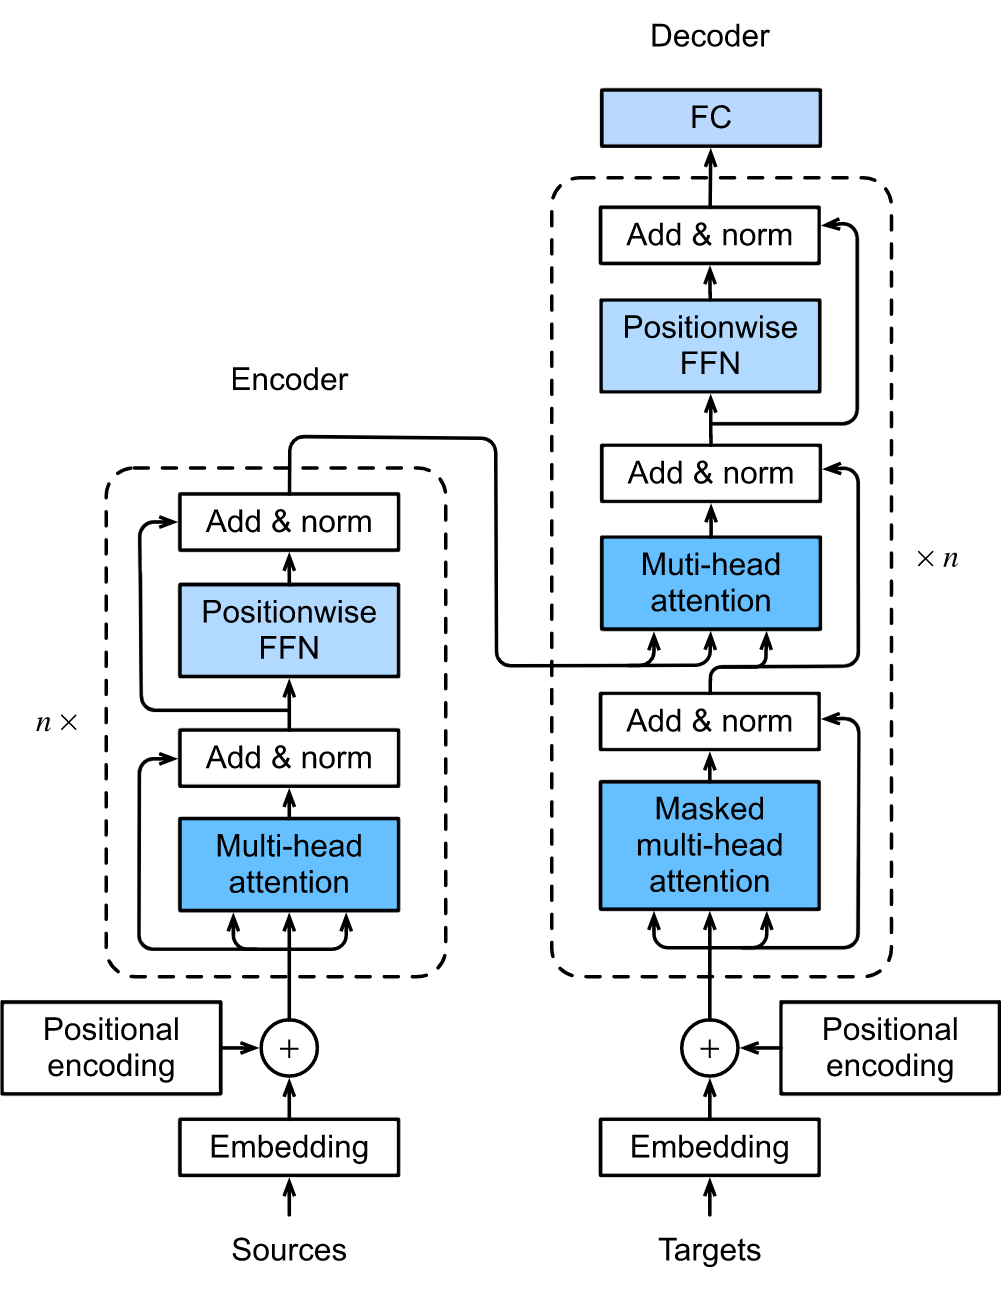
\includegraphics[width=10cm]{figure/TransformerArch.png}
\end{center}
Encoder与Decoder的结构是相似的,只是多了一层Attention。需要强调的是,Encoder的最终输出要送往Decoder的每一层。

下图对照之前的参数结构,给出Encoder一层的结构,没有画出BatchNorm层:
\begin{center}
\includegraphics[width=12cm]{figure/Transformer.png}
\end{center}

大致上是分两部分,首先是Attention层,再加上Linear层。Attention会把输入复制一下送到不同的head和$Q,K,V$。本质上是矩阵乘法、拼接。

其中FF层是
\begin{empheq}{equation*}
\by=W_2\max(0, W_1\bx+\bm{b}_1)+\bm{b}_2
\end{empheq}
现在对照之前的列表,即可看出,$W_1$是$d_{\text{model}}\times d_{\text{ff}}$,对应之前的$10\times 200=2000$,再加上偏移即可。$W_2$是$d_{\text{ff}}\times d_{\text{model}}$,也是2000。

从图中也可以看出,输入和输出的$C$必定等于模型的$d_{\text{model}}$,并且$d_{\text{model}}$必定整除\texttt{nhead}。

对于时间序列模型,输入通常有多个维度,但输出是1,即预测。此时一种直观的做法就是把输出进行复制,但不清楚这样是否合理。但这样一来,$Q,K,V$使用的参数就非常少,比如$C=5$,\texttt{nhead=1},则$Q$对应参数为$5\times 5=25$。或者还可以手动复制,比如5复制4份,得到$C=20$,增加参数数量。

此外,时间序列时用自变量预测因变量,可以把自变量的旧值作为Encoder输入,因变量的新值作为Decoder输入,然后下一时期的值作为输出。
\subsubsection{对比LSTM}
与LSTM相比,Transformer最大的差异就是没有维护内部状态,LSTM中是用$\bm{h,c}$来维护内部状态的。
\section{实践经验}
\subsection{最佳实践}
\begin{enumerate}
\item 使用残差连接。残差网络的性能比一般的网络稍好。但在训练过程中损失函数可能出现阶段式下降的情况,比如在某一阶段几次迭代过程中改变很小,之后才继续下降。尚不明确原因。

在回归中使用残差连接的一种方式就是LSTM+MLP+残差连接。在一次GAN-LSTM实践中,观察到在生成器中使用比LSTM+MLP的效果更好,如果只使LSTM+MLP,那么在MSE在降到最低点几百以后很快会上升,但残差连接不易出现这种情况,稳定性好。

不过残差网络在参数量相似的情况下,运行似乎有点慢。

\item 使用\texttt{gelu, leaky\_relu}一类的损失函数。
\item 使用$3\times3$的卷积核。卷积核不能太大.小的卷积核精度更高,大的卷积核容易丢失信息,一次实验中,使用10层卷积网络,核大小为5,一直只有0.5\%正确率,但降低为$3\times 3$后准确率立即提高了很多.
\item 多网络训练的同步问题.包括GAN之类的网络是由多个网络构成的,需要注意训练时的同步。主要是学习率需要好好设置,一般来说,更加关心的应该学习率设得高一些,比如GAN中的生成器,它的学习率可以设成判别器的10倍,此时相当于把生成器作为主要目标,而判别器作为辅助。GAN中判别器不能太强,也与网络的原理有关,如果判别器太强,则梯度很接近0,没法更新生成器。
\end{enumerate}


\subsection{不能随意使用卷积与ReLU}
在CV中,卷积通常可以起到边缘检测的作用,这要求数据在某个边界发生大的变动.同时ReLU会让很多数据归0,因此假如原本的数据变动不大(比如金融数据),而且有一定随机性,那么套上卷积与ReLU后,很容易使得结果归0.有人据此也认为ReLU函数发挥作用主要是因为正则化.假如此时加上一层全连接,那么起作用的实际上是bias,其它都归0了.

当然,归0也与参数的初始化方式有关,比如Pytorch中默认是均匀分布.大约有一半是负数,可能就比较容易全0.

为了防止归0,可以使用负数部分不归零的函数如PReLU、RReLU.


\subsection{BatchNorm}
使用BatchNorm可以降低损失函数的值,否则层层放大,可能导致损失函数异常大.有的网络中对每一层卷积都用了BatchNorm,可能过于频繁了,两层或更多加一个BatchNorm可能比较好.但BatchNorm本身对最终结果影响不大,只是如果不用的话,可能导致损失函数异常地大.

在一次分类实验中,如果不加BN,网络似乎一直无法训练,准确率一直不变。所以相比之下,还是要使用BN.

在一次回归中,没有使用BatchNorm,好像效果也挺不错,没有出现极端异常的输出。

所以整体上看,分类可以用BatchNorm,回归似乎并不需要。因为分类任务中\texttt{softmax}需要进行指数运算,如果值太大,就会溢出。从这点来看,分类任务中使中$\ReLU$也是有必要的,因为假如值太小,输出归0,就无法训练。
\subsection{评估网络规模与深度}
resnet18有1600万参数,用来给10575个人脸,50万张图片分类绰绰有余.在实际应用中需要注意参数的效率问题,常见的神经网络虽然参数很多,但很多是冗余的,效率不一定高。所以评估需要使用多少参数时,不能只看绝对比例,也要与问题匹配。大致上可能最多取数量的50\%。

在相同的参数下,深度比广度更加重要一些,所以务必要保证深度,尤其是使用relu激活函数时,如果深度不够,很可能出现全0的输出,导致训练很不容易。一般至少要5层以上。

此外,网络深度可能与指数增长有关。假如一个函数是指数增长的,则需要比较深的网络。宽度只相当于标量乘法,比如$x+2x$,而增加深度,就可以带来指数增长,比如$2\times(2 x)=2^2x$。但需要注意的是,这里的“指数增长”不是真正的指数增长,如果想要真正的指数增长,就需要使用$\exp$基函数。在涉及时间序列的预测的时候,“指数增长”性质尤为重要。因为给定的样本可能没有增长那么快,而拟合的时候就只是在拟合标量乘法,所以在样本外预测的时候,增长就不够。增加深度,可以近似指数增长,提高样本外预测的效率。

举一个一元回归的例子,如果只有一层,那么就是线性回归,无论使用多少个参数。假如使用2层,就是二次回归,使用3层,就是三次回归。显然精度会增加。

Transformer中使用了混合类型(\ref{neural-network-basis-function})与混合类型的内积运算,自然地带有指数增长结构。LSTM中也有使用混合类型与内积,但由于使用了激活函数,限定了范围,所以是没有指数增长结构的。

\subsection{直接正则化不一定必要}
很多操作都可以归结为正则化,但就实践的情况来看,使用\texttt{weight\_decay}正则化似乎是没有必要的,效果不明显。

\subsection{学习率不是越低越好}
低学习率更稳定,这是肯定的。但\circled{1}低学习率意味着每次调整的程度很小,那么容易受到初始值的影响,假如初始值不好,那么可能一直在很差的地方徘徊。\circled{2}高学习率也可以是稳定的。高学习率下,可能出现这种情况,就是准确率改变不大,这可能是由于按Batch调整的,很快就调整到最优了。

实践中可以取学习率衰减,范围在1e-1$\sim$1e-7的范围中取。
\subsection{结构改变重于重复运行}
同一个模型,重复运行的结果可能有所区别,但取平均后差别不大。所以主要在于结构和学习率。从这个角度上说,神经网络不完全是玄学。假如每次训练的结果相差非常多,更可能是因为结构或者编程问题。

其基本原理就是对称性,神经网络中蕴含了非常丰富的对称性,所以从不同初始值出发,可能最终的参数不一样,但参数的效果基本上应该是相同的。

但在一次回归任务中,重复运行确实有可能改善运行结果,所以可以多试几次看结果。比如第一次运行执行了400000次迭代验证集上才到达700,但另一次运行只用了13000次次迭代就到了400。不过训练集上损失函数的趋势倒是基本很像,均一直下降,只是测试集上的区别比较大:比如第二次运行中,训练集上MSE从10下降到7时,测试集上MSE从500变成800,但中途出现了200的训练集MSE波动较大。

究其原因,可能与随机Batch有关。有些样本可能本身比较难学习,随机采样时优先学到了这样的样本,可能学习起来就不容易,第二个原因是样本的非对称性,首先学习一种样本,再学习另一种,效果并不一样。


\subsection{一些现象}
\begin{enumerate}
\item 假如准确率前期一直不变,然后增加。这可能是由于学习率太低,造成每次改进很小,就不影响准确率。
\item 假如准确率一直不变(区别上一条),可能是学习率太高,分类任务中,可以取1e-6。
\item 全连接网络,似乎不一定越深越好,一次实验中,3+4层可能一直没法训练,而换成2+4就变好了,但这种好还是跟偶然性有关的。
\item 三分类任务,测试准确率一开始很高,然后稳定下降到1/3左右,一直不变。这个现象的原因可能是由于\texttt{weight\_decay}。它的设置为
\begin{verbatim}
torch.optim.Adam(parms1,lr=1e-5, weight_decay=1e-3)
\end{verbatim}
可能由于\texttt{weight\_dacay}比较大,所以后期导数的调整作用失效了。如果完全去掉,准确率可以一直上升。
\item 训练集上正确率一开始就是1,很可能就是过拟合了。另一方面,如果神经网络可以很快学到,说明数据本身可能比较简单。通过对抗式学习可以缓解过拟合,但这种网络不容易训练。
\item 网络的输出可能一开始变化非常小,比如只变动0.01,但经过训练之后,可能运动到变化非常大的区域,此时可能一下子从-1变到4.相当于从很平坦的区域运动到很陡峭的区域,尚不明确原因。
\end{enumerate}
